\documentclass[xcolor=table]{beamer}

\usetheme[secheader,compress]{Madrid} %Primary theme

\usepackage{verbatim}
\usepackage{graphicx}
\usepackage{tcolorbox}
%% UTM Colors
\definecolor{UTMblue}{rgb}{0.043137, 0.137254, 0.254901}
\definecolor{UTMorange}{rgb}{1.0, 0.509803, 0}

\setbeamercolor{palette primary}{bg=UTMblue,fg=white}
\setbeamercolor{palette secondary}{bg=UTMblue,fg=white}
\setbeamercolor{palette tertiary}{bg=UTMblue,fg=white}
\setbeamercolor{palette quaternary}{bg=UTMblue,fg=white}
\setbeamercolor{structure}{fg=UTMblue} % itemize, enumerate, etc
\setbeamercolor{section in toc}{fg=UTMblue} % TOC sections
\setbeamercolor{title}{fg=UTMorange}
\setbeamercolor{subsection in head/foot}{bg=UTMorange,fg=white}


\setbeamertemplate{footline}
{
  \leavevmode%
  \hbox{%
    \begin{beamercolorbox}[wd=.33\paperwidth,ht=2.25ex,dp=1ex,center]{author in head/foot}%
      \usebeamerfont{author in head/foot} J.~Chamberlain \& A.~Lum
    \end{beamercolorbox}%
    \begin{beamercolorbox}[wd=.44\paperwidth,ht=2.25ex,dp=1ex,center]{title in head/foot}%
      \usebeamerfont{title in head/foot}%
      \parbox{\linewidth}{\centering Revitalizing Solar Insights: A Dashboard for WTSF}
    \end{beamercolorbox}%
    \begin{beamercolorbox}[wd=.23\paperwidth,ht=2.25ex,dp=1ex,right]{date in head/foot}%
      \usebeamerfont{date in head/foot} \insertdate \hspace*{1em} \insertframenumber{} / \inserttotalframenumber\hspace*{1ex}
    \end{beamercolorbox}%
  }%
  \vskip0pt%
}


%\setbeamertemplate{footline}
%%%%%%%%%%% BEGIN MACROS %%%%%%%%%%%%%%%%%%
% frameT: Frame with title
\newcommand{\frameT}[2]{\frame{\frametitle{#1} #2}}

% frameF: Fragile frame with title
\newcommand{\frameF}[2]{
  \begin{frame}[fragile]
    \frametitle{#1}
    #2
  \end{frame}
}

% frameTop: Frame aligned t the top
\newcommand{\frameTop}[2]{\frame[t]{\frametitle{#1} #2}}


\newcommand{\tab}{\hspace{1cm}}

\newcommand{\spaceor}{\hspace{5pt} \textbf{or} \hspace{5pt}}

%%%%%%%%%%% END MACROS %%%%%%%%%%%%%%%%%%%%

\begin{document}

\title{Revitalizing Solar Insights: A Dashboard for West Tennessee Solar Farm}

\author{Joshua Chamberlain \& Andy Lum \\ \vspace{0.1in} Mentor: Dr.~Justin R.~Sims}
\institute{UT Martin}
\date{\today}



\frame{\titlepage}
\begin{frame}[c] % Use [c] to center the content vertically
%%%%%%%%%%%%%%%%%%%%%%%%%%%%%%%%%
%
%   TABLE OF CONTENTS           %
%
%%%%%%%%%%%%%%%%%%%%%%%%%%%%%%%%%
\frametitle{Table of Contents} 
\begin{enumerate}
    \item<1-> Introduction
    \begin{itemize}
        \item<2-> Motivation
    \end{itemize}

    \item<3-> R-Shiny \& Functionalities
    \begin{itemize}
        \item<4-> What is R-Shiny?
        \item<5-> Functionalities
    \end{itemize}

    \item<6-> List of Technologies
    \begin{itemize}
        \item<7-> Technologies used to supply the dashboard
    \end{itemize}

    \item<8-> Project Goals
    \begin{itemize}
        \item<9-> What do we want to accomplish overall?
    \end{itemize}

    \item<10-> Dashboard Demo

    \item<11-> Results
    %\begin{itemize}
        %\item<12-> What went well? What didn't go well?
    %\end{itemize}

    \item<12-> Conclusion
    %\begin{itemize}
        %\item<14-> What did we accomplish? What did we learn?
    %\end{itemize}

    \item<13-> Future Work

    \item<14-> Contact Information
\end{enumerate}
\end{frame}

%%%%%%%%%%%%%%%%%%%%%%%%%%%%%%%%%
%
%   INTRODUCTION / MOTIVATION   %
%
%%%%%%%%%%%%%%%%%%%%%%%%%%%%%%%%%
\frameT{Introduction}{
    \vfill 
    \begin{block}{Motivation}
     Can we build an interactive dashboard to improve research and education accessibility, optimize power production, and advance sustainable energy practices?
    \end{block}
    \vfill
}

%%%%%%%%%%%%%%%%%%%%%%%%%%%%%%%%%
%
%   R-SHINY & FUNCTIONALITIES   %
%
%%%%%%%%%%%%%%%%%%%%%%%%%%%%%%%%%
\section{}
\frameT{R-Shiny \& Functionalities}{
    \begin{enumerate}
        \item<1-> Provides an easier and more integrated way to creating web-based dashboards without needing to learn web development languages like HTML.
        \item<2-> Provides the following functionalities:
        \begin{itemize}
            \item<3-> Real-Time Data Visualization
            \item<4-> Interactive Maps
            \item<5-> Sensor Information Panel
            \item<6-> Historical Data Analysis
            \item<7-> User-Friendly Interface
            \item<8-> Responsive Design
            \item<9-> Dashboard Hosting
            \item<10-> Export Data
        \end{itemize}
    \end{enumerate}
}

%%%%%%%%%%%%%%%%%%%%%%%%%%%%%%%%%
%
%   LIST OF TECHNOLOGIES        %
%
%%%%%%%%%%%%%%%%%%%%%%%%%%%%%%%%%
\section{}
\frameT{List of Technologies}{
  \begin{enumerate}
      \item<1-> \textbf{MySQL}\par
      stores and manages sensor data in a table containing minute by minute data separated by data for each sensor.
      \item<2-> \textbf{Python}\par
      Retrieves data from the MySQL database and updates a Google Drive CSV for data simulation.
      \item<3-> \textbf{R-Shiny}\par
      Develops an interactive dashboard for data visualization.
      \item<4-> \textbf{Shinyapps.io}\par
      Hosts a web server to allow users from all major operating systems to be able to access the dashboard.
      \item<5-> \textbf{Google Cloud Console}\par
      Safeguards API information for enhanced data security.
  \end{enumerate}
}
%%%%%%%%%%%%%%%%%%%%%%%%%%%%%%%%%
%
%   PROJECT GOALS               %
%
%%%%%%%%%%%%%%%%%%%%%%%%%%%%%%%%%
\section{}
\frameT{Project Goals} {
  \begin{enumerate}
      \item<1-> \textbf{Streamlined Data Pipeline}
      %Achieve efficiency by establishing a robust data pipeline from MySQL to Python, culminating in organized data storage within Google Drive's CSV format, seamlessly facilitating further analysis within the R-Shiny environment.
      \item<2-> \textbf{Continuous Data Maintenance}
      %Elevate data integrity through the implementation of an automated Python script, equipped with comprehensive error handling capabilities, ensuring the continuous and real-time updating of Google Drive's CSV repository to provide a reactive data environment.
      \item<3-> \textbf{R-Shiny Dashboard}\par
      encompasses all of the aforementioned functionalities.
      \item<4-> \textbf{Cross-Platform Accessibility}\par 
      Ensure inclusivity by designing a webpage that accommodates diverse laptop operating systems, guaranteeing a seamless user experience.

        \bigskip
  \end{enumerate}
}
%%%%%%%%%%%%%%%%%%%%%%%%%%%%%%%%%
%
%   DASHBOARD DEMO              %
%
%%%%%%%%%%%%%%%%%%%%%%%%%%%%%%%%%
\frameT{Dashboard Demo} {
  \href{https://seniordesign.shinyapps.io/shiny_dashboard/}{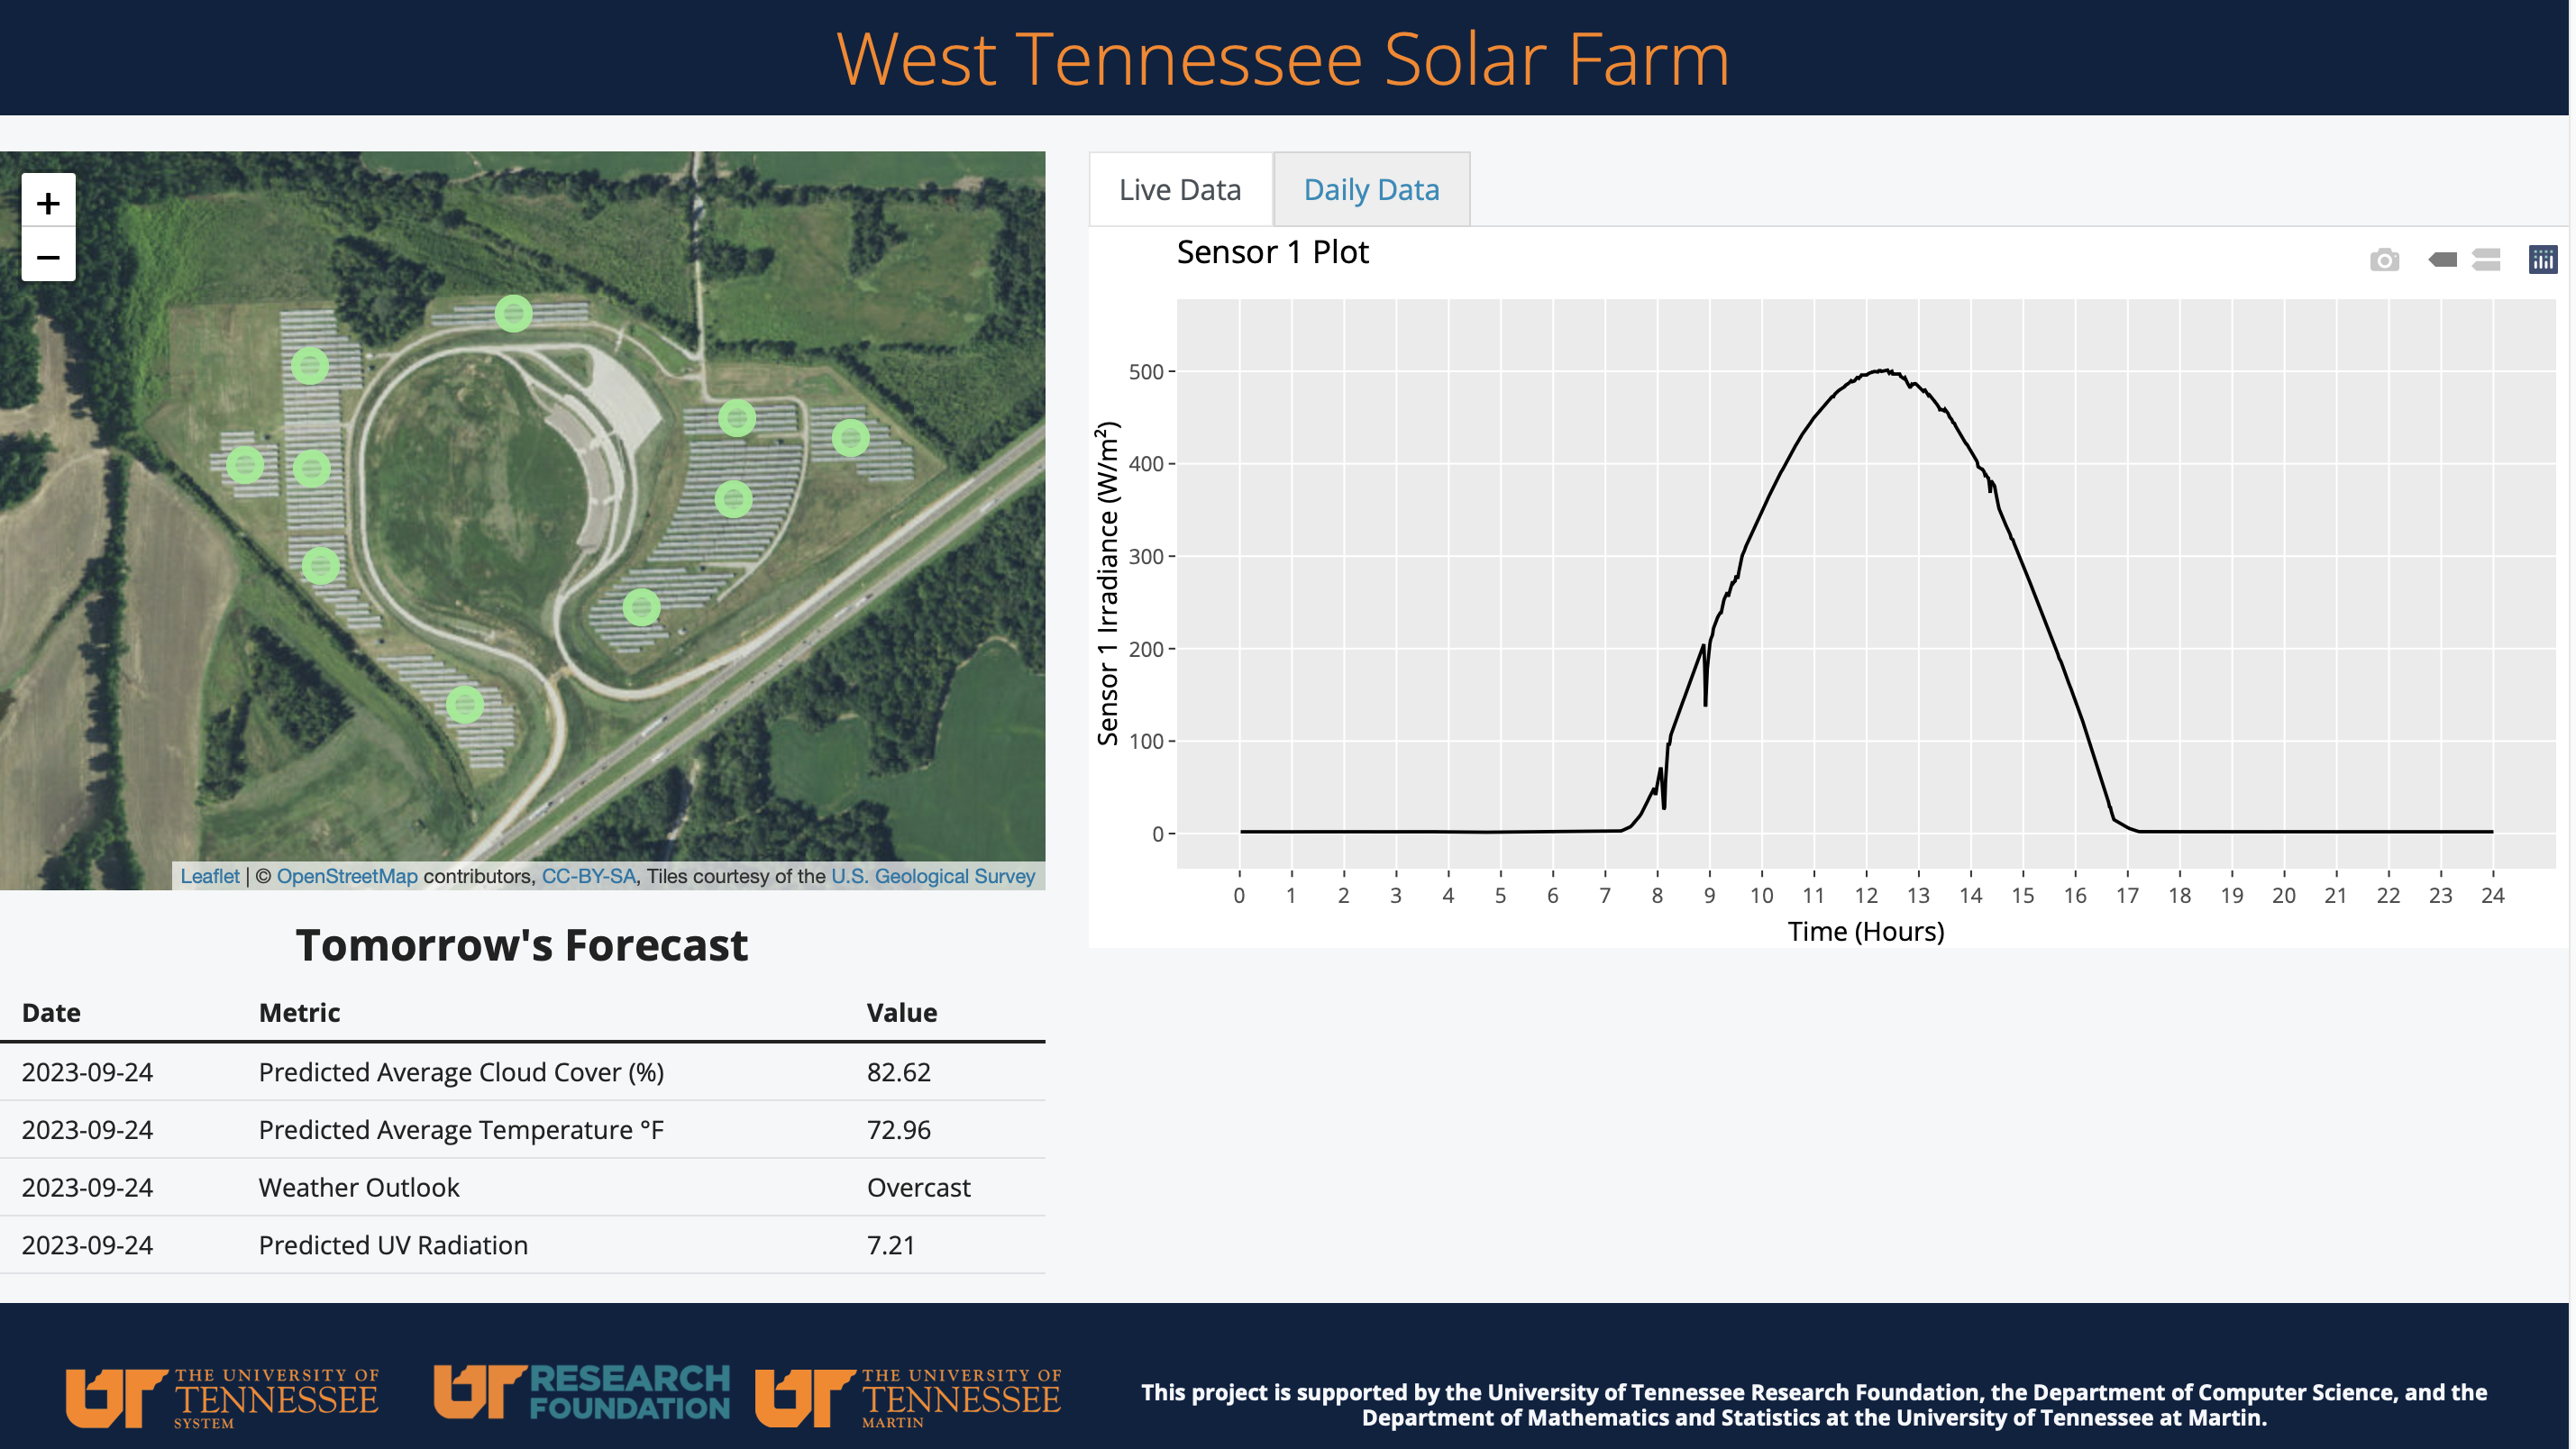
\includegraphics[width=\linewidth]{Dashboard.png}}
}

%%%%%%%%%%%%%%%%%%%%%%%%%%%%%%%%%
%
%   FOR JOSH                    %
%
%%%%%%%%%%%%%%%%%%%%%%%%%%%%%%%%%
\frameT{Future Work} {
    \begin{enumerate}
        \item<1-> \textbf{Predictive Analysis}
        \item<2-> \textbf{Notifications}
        \item<3-> \textbf{Video Tutorial}
    \end{enumerate}
}

\frameT{Conclusion} {
    The dashboard creates:\\
    \begin{enumerate}
        \item An educational tool for people to learn about the Solar Farm Process
        \item A research tool that provides public data to study
    \end{enumerate}
}
% \begin{frame}[fragile]
%   \frametitle{Power Consumption}
%   \begin{figure}[ht]
%     \begin{minipage}[b]{0.53\linewidth}
%       \centering
%       Minipages are a great way to
%     \end{minipage}
%     \hspace{0.5cm}
%     \begin{minipage}[b]{0.4\linewidth}
%       \centering
%       Line up side-by-side content.

%     \end{minipage}
%   \end{figure}
  
% \end{frame}

% \section{Results}
% \frameT{Results} {
%   Describe any results of your work here.

%   \bigskip

%   Things that worked?

%   \bigskip

%   Things that didn't work?
% }
% \section{Conclusion}
% \frameT{Conclusions} {
%   Some bullet points here to wrap things up.
% }
\section{Contact Information}
\frameT{Any Questions?} {
  

  \begin{center}
    Comments?
  \end{center}

  \bigskip

  \textbf{Joshua Chamberlain}: \href{mailto:jospcham@ut.utm.edu}{jospcham@ut.utm.edu}.
  \bigskip
  
  \textbf{Andy Lum}: \href{mailto:andlum@ut.utm.edu}{andlum@ut.utm.edu}.
  \begin{center}
    %\includegraphics[width=4cm]%{figures/6AnLddq.png}
  \end{center}
}
\end{document}